\documentclass[10pt]{article}
\usepackage[utf8]{inputenc}
\usepackage{grafematik}

\title{Malayalam Orthographic Reforms: \\Impact on Language and Popular Culture}

\author{Santhosh Thottingal \\
 Swathanthra Malayalam Computing \\
 {\small {\tt santhosh.thottingal@gmail.com}} \\
 \and
 Kavya Manohar \\
 Swathanthra Malayalam Computing \\
 {\small {\tt sakhi.kavya@gmail.com}}}

\date{}

%\date{October 2017}

\begin{document}

\maketitle

\begin{abstract}

Malayalam is a language spoken in India, predominantly in the state of Kerala with about 38 million native speakers. The Malayalam script evolved from Brahmi through Grantha lipi and Vattezhuthu writing systems. The script orthography has acquired its uniqueness with its complex shaped graphemes formed by the combination of consonant sequences and  signed vowel forms. The number of unique graphemes in this system exceeds fifteen hundred. The orthographic styles were constantly evolving. In 1971 there was a Governmental intervention in the orthograhy, to reduce its complexity to minimise the labour on typesetting and printing. This paper is an attempt to bring out the impact of this orthographic reforms on various aspects of script usage including popular culture, media, textbooks, graffiti and handwriting. It will also analyse the impact of Unicode and the advancement in digital typography on the orthographic diversity of Malayalam script.

\end{abstract}
 \textbf{Keywords:} Malayalam Script, Orthography Reforms, Unicode, Graphemes

\section{Introduction}

\paragraph{}

With 38 million native speakers Malayalam is the official language of the state of Kerala, India.  Malayalam used to be written in Vattezhuthu, a script for Tamil, another south Indian language. The modern Malayalam script evolved from Grantha alphabet which was a script for Sanskrit. Both Vattezhuthu and Grantha has its roots in the Brahmi script\cite{}. The modern Malayalam script has 15 vowels and 36 consonants as the basic character set. The vowels have signed notations to be used with consonants.

\paragraph{}
The script is mainly abugida, or alphasyllabary. That is, consonant–vowel sequences are written as a unit: each unit is based on a consonant or conjunct letter, and vowel notation is secondary. Vowels have independent existence, but only at word beginnings. This is the common characterestic of  Brahmic family of scripts of South and Southeast Asia\cite{}.

\paragraph{}
The script has acquired its uniqueness with its complex shaped ligatures formed by the consonants and conjuncts with signed vowel forms. Conjuncts are formed by a sequence of two more consonants. The conjunct grapheme usually has a shape smoothly blend from the constituent consonants. The Orthographic styles were continuously evolving. The shapes of conjuncts, relative positioning of signs and their sizes have changed over time to match the needs of writing schemes. Stylus on dry leaves gave limited flexibility and the graphemes were rarely perfect rounds. But pen on paper made it more curvy.

\paragraph{}
When printing technology started getting popular there was a requirement to cast movable types in huge numbers. Even though the basic characters were less than hundred, the orthographic style demanded separate types for conjuncts, and their signed vowel forms. Apart from vowels, some consonants too have signed notations, further increasing the number of types needed in the foundry. The first printed book in Malayalam, \begingroup \manjari സംക്ഷെപവെദാർത്ഥം \endgroup in 1772 had more than thousand unique types \cite{}. The manual labour on typesetting and lay outing were high for the same reason. The script continued to evolve by separating some vowel sign types (\begingroup \manjari{   ി, ീ } \endgroup) from the consonant/conjunct grapheme . The early typographers of Malayalam script made the curvy style of the orthography popular. 

\paragraph{}
In 1971, there was a governmental order by the state of Kerala intended to reduce the complexity of the script. The proposal was to discard the usage of complex conjuncts and to separate the vowel notations from the consonants/conjuncts.  The orthography  reformation proposal was to reduce the challenges imposed by the script on the typesetting and printing technology. Being a forced intervention, this was a major event to be marked in the history of the orthographic evolution. 

\paragraph{}
Still, the traditional complex orthography continues to be used in wall graffiti, poster designs and handwriting. The print media, publishing industry  and text books switched to the reformed orthography to varying extends. Publishers adopted a set of conjuncts as per their choice. The set never strictly stuck to the reformation order. But the vowel signs mostly got separated from the conjuncts. 

\paragraph{}
The digitization of printing was yet another remarkable event. The pre-Unicode digital fonts in Malayalam were Malayalam letters mapped to the ASCII character space.  Such fonts retained only a limited repertoire of conjuncts. Also the signed notations of vowels and consonants were detached from the base grapheme. Digital fonts before the unicode era embraced the reformed orthography more closely. The publishing industry largely depended on these fonts for decades.


\paragraph{}
With the advent of Unicode based digital typography, complex conjunct formations and their rendering were no more a technological challenge. With only the basic graphemes  encoded in Unicode, any long sequence of consonants and signs could be mapped to a single conjunct grapheme in signed or unsigned form.  Complex rendering rules of the script can easily be handled by modern rendering engines. With these technical advancements, fonts which could very well support the traditional orthographic scheme of the Malayalam script emerged. The usage spans from movie titles to news portals and periodicals.

\paragraph{}
Today the script in the popular culture is a mix of traditional as well as the reformed style. The paper analyses the impact of Unicode and the advancement in digital typography on the orthographic diversity of Malayalam script. We will analyse the evolutionary path of the script as well.


\section{Script and the nature of graphemes}

\begin{itemize}
\item
Vowels and consonants are the basic building blocks of Malayalam script.
\item
 Vowels have stand alone existence in their pure form. 
\item
Alternately vowels also appear as signed form modifying a consonant sound, vowel signs have no existance  without a consonant. 
\item Consonants in Malayalam always have the inherent vowel /a/ present in them.
\item
 Any other vowels sound associated with a consonant is written as a signed form of the consonant. The signs can be prebase, postbase or both. Some signs modify the shape of base grapheme.
\item
The removal of inherent /a/ in a consonant is marked in the script by a special character \textit{virama}. 
\item
Virama after a consonant not only removes inherent /a/ but also indicate no vowel sound follows it. 
\item
A conjunct is formed when a consonant follows a sequence of consonant and virama.
\item
 A conjunct can also be formed by a consonant which follows a sequence of conjunct and virama. Every conjunct can be modified by a vowel sign.  
\item
Some consonats at the end of conjuncts have signed forms. eg: \manjari{  ്‌ര, ്‌ല, ്‌യ  }

\end{itemize}



All these cases of complex grapheme formation are exemplified in the table below.
\newline

\manjari

{

\begin{tabular}{|c|c|c|c|}
\hline
അ  &  pure vowel (No explicit  vowel sign ) & &/a/ \\
\hline
ആ  &  pure vowel && /aː/ \\
\hline
ാ & vowel sign of ആ  &Never exist alone &   /aː/ \\  
\hline
ു & vowel sign of ഉ &(Never exist alone) &  /u/ \\
\hline
ഗ &  consonant & No sign attached. Has inherent /a/  & /ga/  \\
\hline
ഗാ & Consonant with vowel sign of ആ&  &  /ga/  \\  
\hline
ഗു & Consonant with vowel sign of ഉ &  & /gu/  \\ 
\hline
് & The virama mark.&Removes the inherent /a/ from vowels & \\
\hline
ഗ് & Consonant ഗ with the virama mark& & /g/ \\
\hline
ഗ്ദ  & consonant, virama, consonant & ഗ,്,ദ &  / ɡd̪a/  \\
\hline
ഗ്ദു & c\_virama\_c vowelsign & ഗ,്, ദ, ു & /ɡd̪u/ \\
\hline
ഗ്ദ്ധ   & c\_virama\_c\_virama\_c   & ഗ,്,ദ,്,ധ  & / ɡd̪d̪ʱa/  \\ 
\hline
ഗ്ദ്ധു &  c\_virama\_c\_virama\_c  &  ഗ,്,ദ,്,ധ ,ു  &  /   ɡd̪d̪ʱu/ \\
\hline
ഗ്ര & c\_v\_c ( signed form)  &  ഗ,്,ര (end consonant is ര ) & /gu/  \\ 
\hline


\end{tabular}

}

The 

\begin{figure}[h]
  \centering
   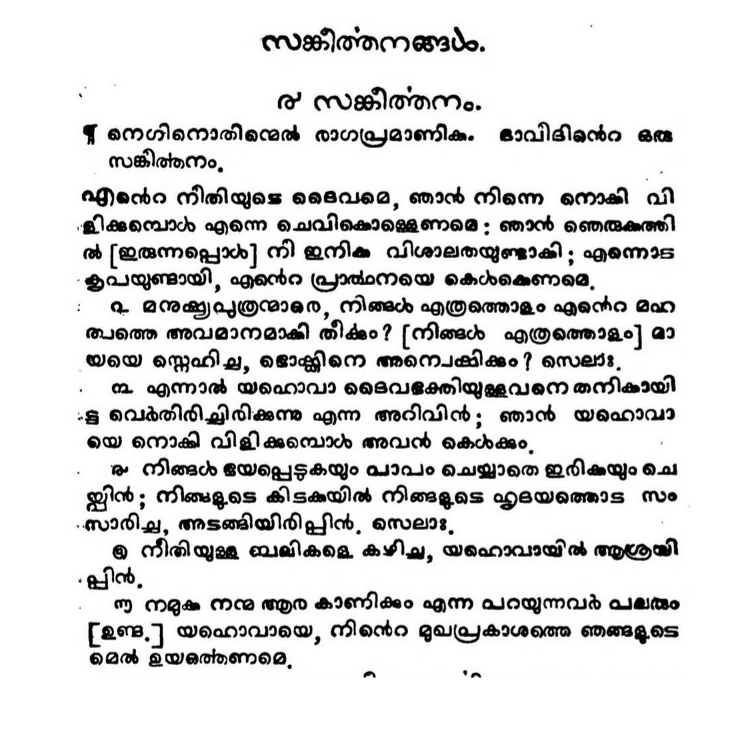
\includegraphics[scale=0.5]{images/1839-Book-of-psalms.png}
     \caption{1839}
\end{figure}

\begin{figure}[h]
  \centering
   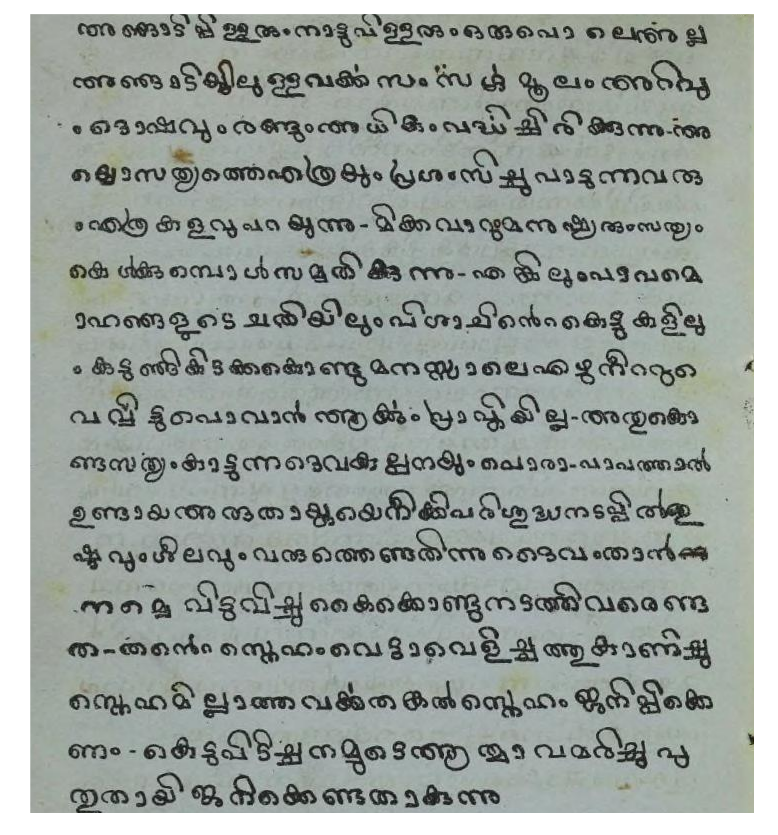
\includegraphics[width=1.0\textwidth]{images/1845-Pazhancholmala-Gundert.png}
     \caption{1845}
\end{figure}

\begin{figure}[h]
  \centering
   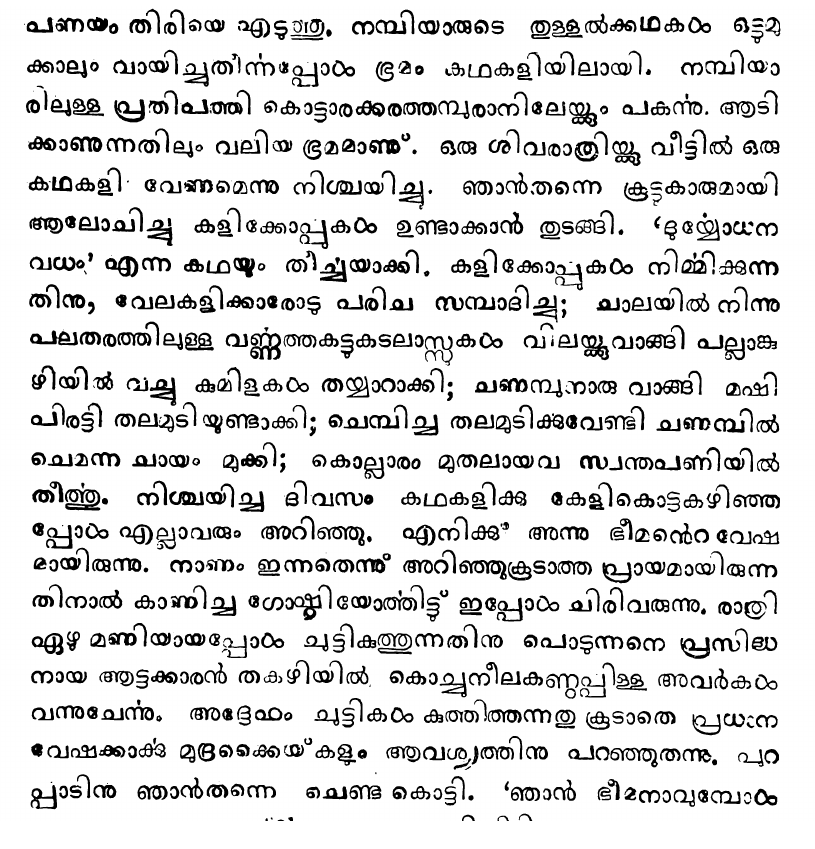
\includegraphics[width=1.0\textwidth]{images/1930-Sabdatharavali.png}
     \caption{1930}
\end{figure}


\begin{figure}[h]
  \centering
   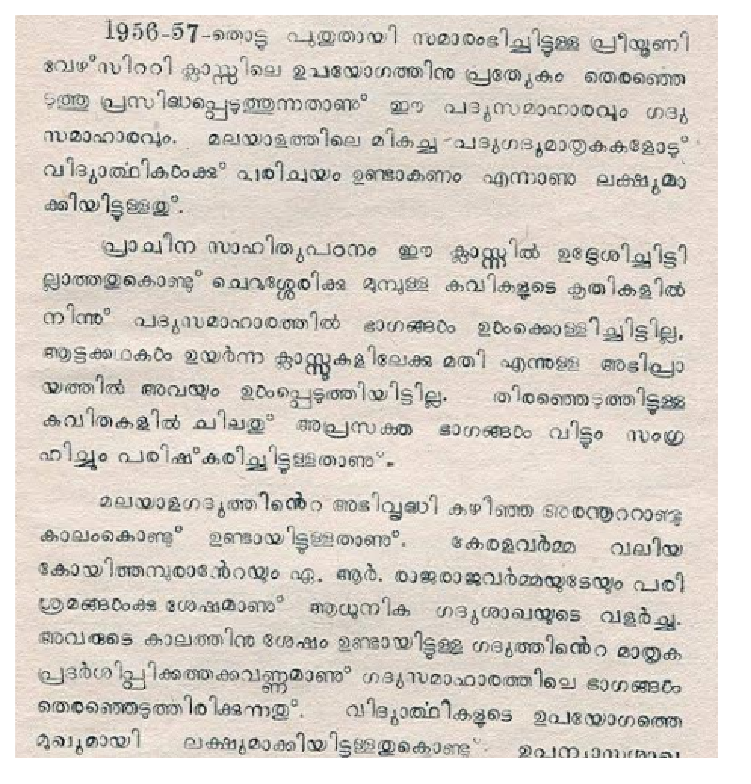
\includegraphics[width=1.0\textwidth]{images/1960-Textbook.png}
     \caption{1960 Malayalam text book}
\end{figure}


\section{Reformation}
Reasons
\begin{figure}
  \centering
   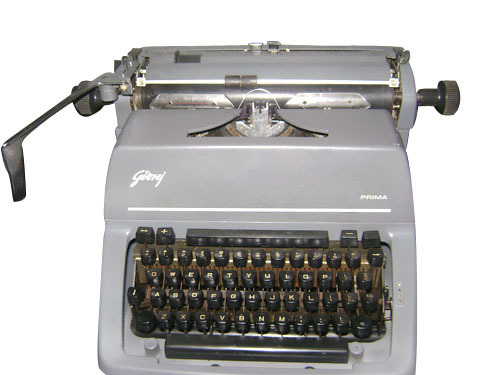
\includegraphics[width=1.0\textwidth]{images/godrej-typewriter.jpg}
     \caption{Godrej typewriter}
\end{figure}

Balu phd aper.

Reformation committee
Govt. Order

\begin{figure}[h]
  \centering
   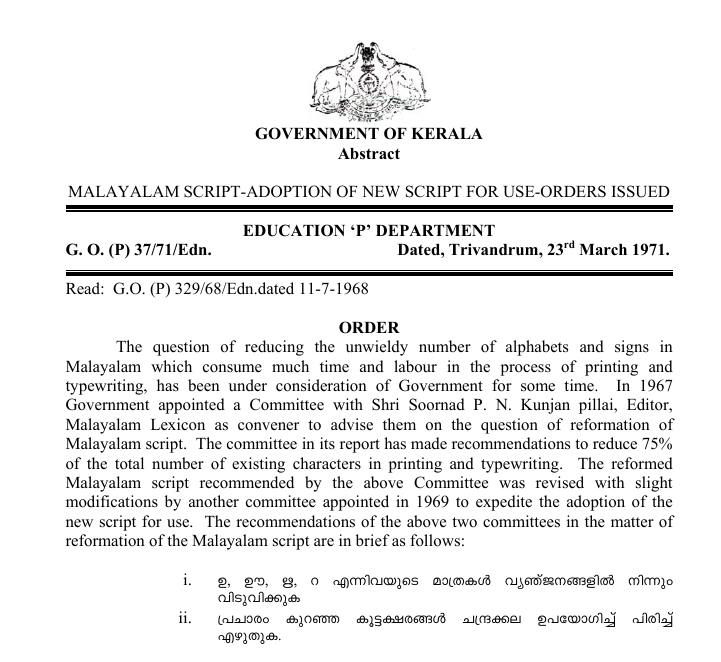
\includegraphics[width=1.0\textwidth]{images/1971-gov-script-reformation-order.png}
     \caption{1971 Govt. order}
\end{figure}

\begin{figure}
  \centering
   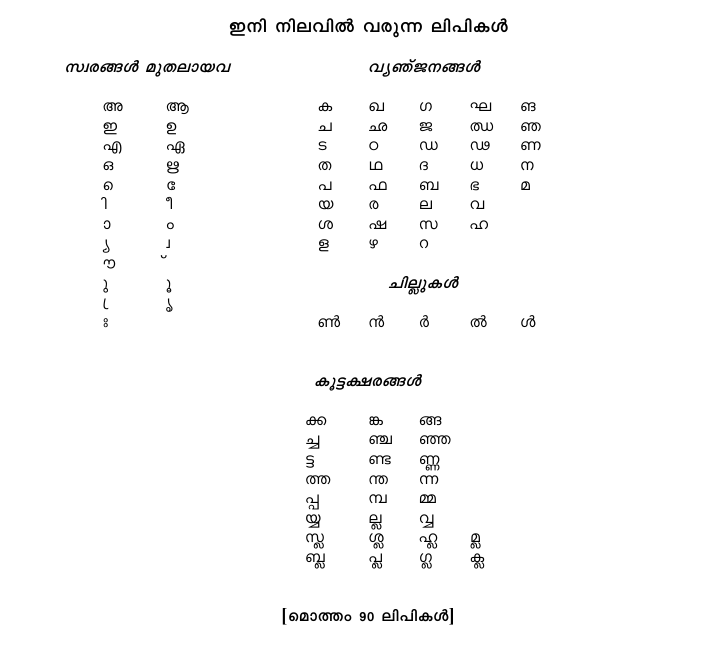
\includegraphics[width=1.0\textwidth]{images/1971-new-lipi.png}
  \caption{New charactors proposal}
\end{figure}

\subsection{Implementation}
Newspapers, Textbooks, Education

\section{Practice}
\subsection{Education}

\begin{figure}
  \centering
   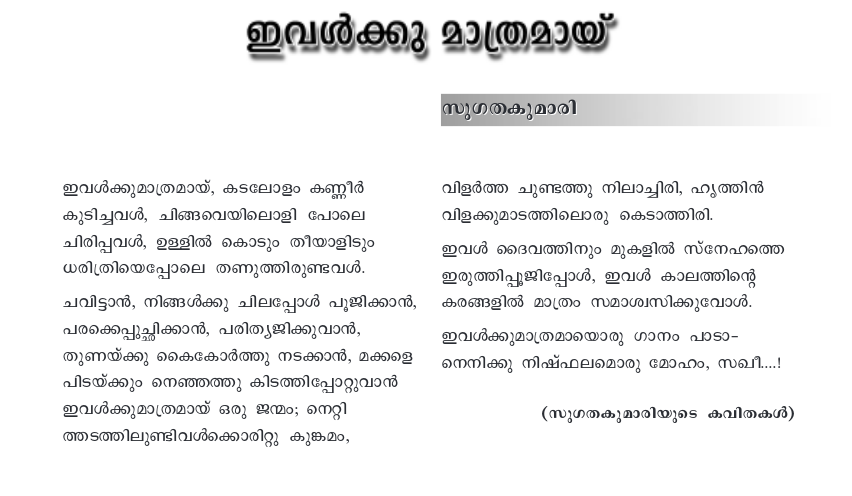
\includegraphics[width=1.0\textwidth]{images/2011-Malayalam-Textbook.png}
     \caption{2011 Malayalam text book}
\end{figure}

\subsection{handwriting}
\subsection{Wall writing}
\subsection{Media}
\begin{figure}
  \centering
   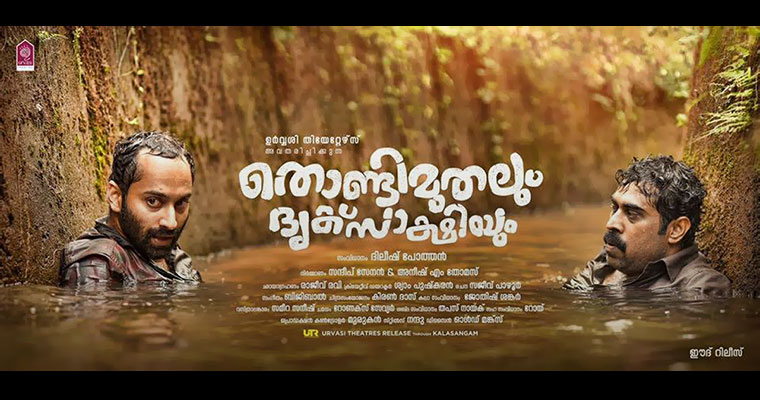
\includegraphics[width=1.0\textwidth]{images/2017-movieposter-Thondimuthal}
  \caption{A Malayalam movie poster from 2017. Uses traditional orthogrophy for title.}
\end{figure}

\begin{figure}
  \centering
   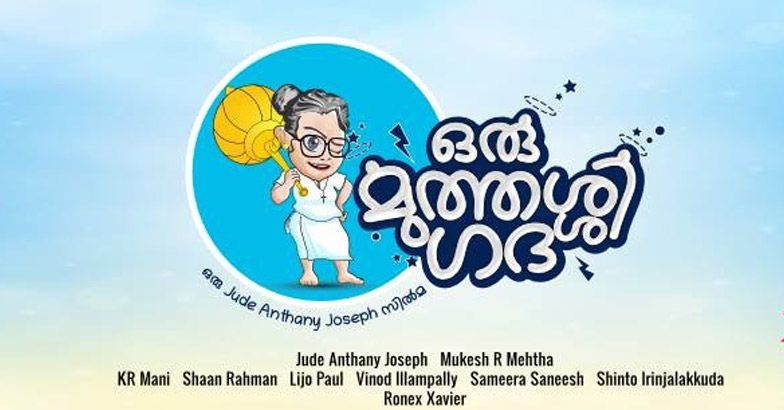
\includegraphics[width=1.0\textwidth]{images/2016-oru-muthashi-gadha}
  \caption{A Malayalam movie poster from 2016. Uses traditional orthogrophy for title.}
\end{figure}

\begin{figure}
  \centering
   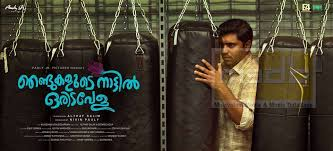
\includegraphics[width=1.0\textwidth]{images/2017-movieposter-njandukalude}
  \caption{A Malayalam movie poster from 2016. Uses traditional orthogrophy for title.}
\end{figure}


\subsection{Internet}

\begin{figure}
  \centering
   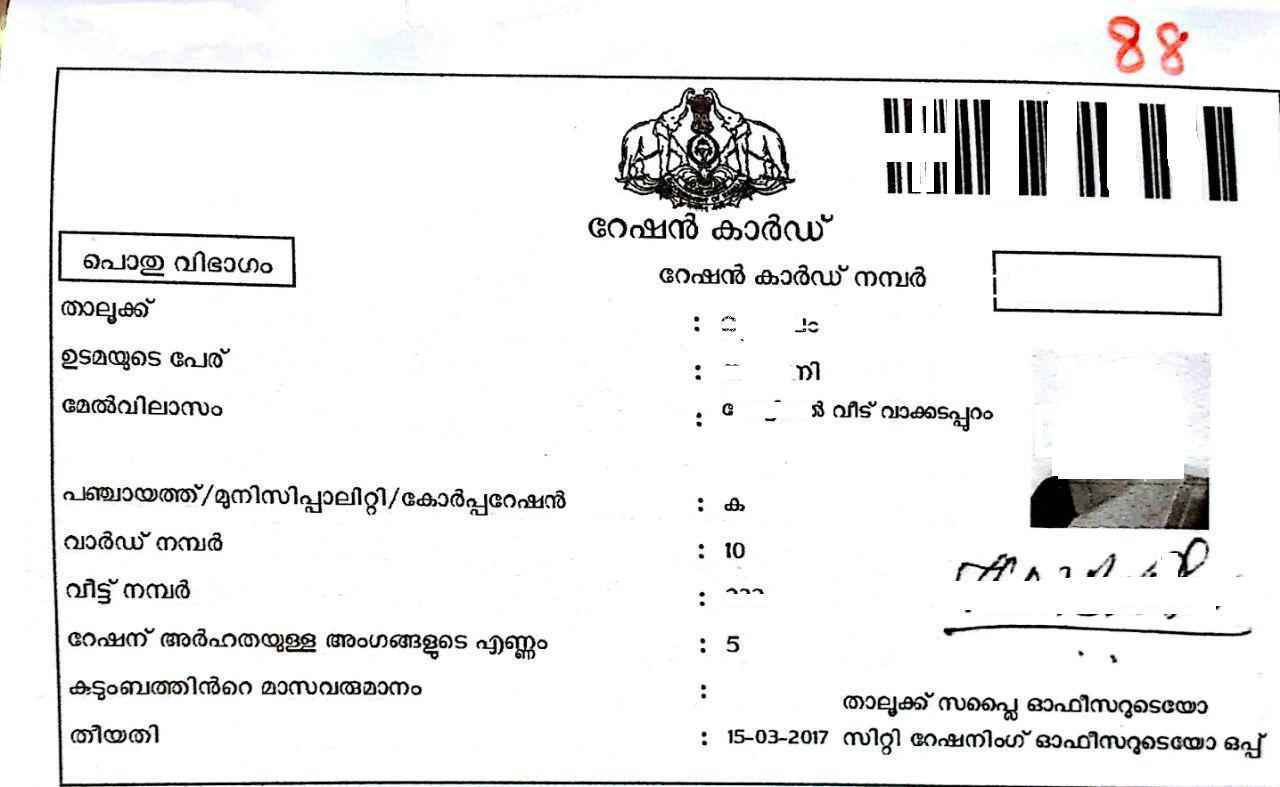
\includegraphics[width=1.0\textwidth]{images/2017-rationcard.jpg}
     \caption{2017 Ration card}
\end{figure}


\begin{figure}
  \centering
   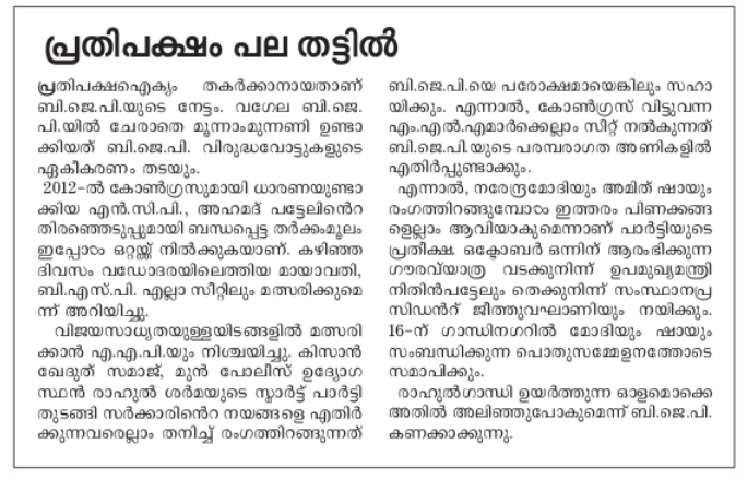
\includegraphics[width=1.0\textwidth]{images/2017-Mathrubhumi-newspaper.png}
     \caption{2017 Mathrubhumi news paper}
\end{figure}


\begin{figure}
  \centering
   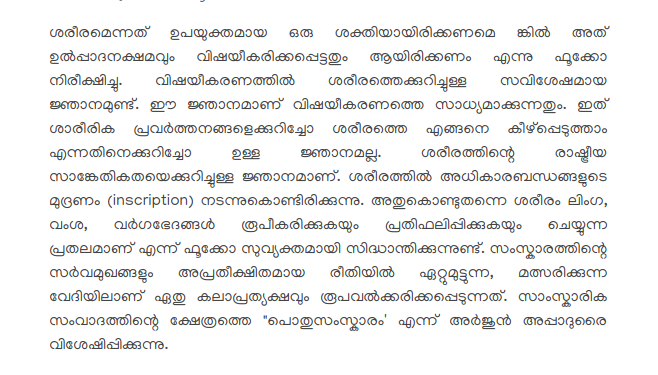
\includegraphics[width=1.0\textwidth]{images/Manjari-Body-Text.png}
     \caption{2017 Manjari font- a widely used unicode font}
\end{figure}

ICU memes

\section{References}

\end{document}
